\section{Gateway Implementation}
Things start to get more interesting and complicated here. The Gateway will have to implement both the MQTT protocol and UART communication, using Python. For the MQTT, in order to keep the project consistent, we will use the \href{https://pypi.org/project/paho-mqtt/}{\textcolor{blue}{paho-mqtt}} package to establish the communication protocol. For the UART serial, we will stick with the popular \href{https://pypi.org/project/pyserial/}{\textcolor{blue}{pyserial}} package.

\subsection{Gateway Overture}
\label{subsection:gtw-overture}
Before getting our hands dirty into the implementation of the Gateway, there are plentiful of things to discuss. We will devote this part of the Gateway section for sketching out the overall activities of our gateway program, as well as explaining some observations of the MQTT on Adafruit server.

\subsubsection{Gateway Features}
The bulk of this python program is to running a simple gateway that is capable of receiving data from the \href{https://io.adafruit.com/}{\textcolor{blue}{Adafruit server}} (broker) and dispatching it to an IoT Arduino node. The gateway also monitors the data sent from the Arduino and publishes it to the server, therefore establishing a form of communication between the broker and the sensor. The attributes of this simple implementation of our gateway are listed bellow.
\begin{itemize}
    \item The gateway receives \textbf{temperature} and \textbf{humidity} data from the Arduino and publishes them to the broker.
    \item The gateway listens to \textbf{led} and \textbf{servo} data from the broker and dispatches them to the Arduino.
    \item The gateway is in charge of the \textbf{gtw-status} topic, which is exclusively reserved for the gateway to declare its status to the broker.
    \item The gateway also maintains a concrete connection with the Arduino. When launch, the gateway must ensure it has successfully communicated with the Arduino before establish the broker-connection. During runtime, if the arduino connection is compromised, the gateway will immediately terminate it activities, cut off its connection with the broker, do any necessary clean-up work, and exit with a warning.
    \item Whenever the gateway makes a successful connection to the broker, whether it is the first time the gateway connects to the server or it is a re-connection attempt due to any failure, it will automatically fetch the latest data from any topic it subscribes to and dispatch them to the Arduino.
\end{itemize}
With these features kept in mind, we can sketch out the behaviour of our gateway activities. The step-by-step implementation will be further demonstrated in later part of this section. In the mean time, it is not redundant to mention some "catches" when we use the Adafruit server in join with the paho-mqtt package.

\subsubsection{Adafruit Limitation}
MQTT is one of the powerful communication protocols, especially in the world of IoT. Since its invention in 1999, the latest MQTT version one can use at the point of writing this document is \href{https://docs.oasis-open.org/mqtt/mqtt/v5.0/mqtt-v5.0.html}{\textcolor{blue}{MQTT v5.0}}. While we can exploit many rich IoT features provided by the latest version of MQTT, that is not the case for the Adafruit broker, which by far supports just the MQTT v3.1.1. Even this version of MQTT is strong enough to handle almost any asspect of IoT communication, the Adafruit broker isolates itself from the standard and provides its own python \href{https://pypi.org/project/adafruit-io/}{\textcolor{blue}{API library}} for the end users. This API package is built as a wrapper of the paho-mqtt library, made possible by the people behind the Adafruit broker, to provide ease of use and discard the features of the standard that the Adafruit server is not capable of. So basically, if we use the paho-mqtt package to implement the MQTT and not the exclusive library offered by the Adafruit developers, some functionality provided by the library will not take effect. This is one significant point that need be kept in mind when doing paho-mqtt in joint with the Adafruit broker.

So what is missing from the Adafruit server? The comprehensive document (published by the Adafruit, of course) can be found \href{https://io.adafruit.com/api/docs/mqtt.html#adafruit-io-mqtt-api}{\textcolor{blue}{here}}. They provide us with the guide to implement MQTT communication to the Adafruit server without using the exclusive package. There are many points to be considered, for example the limit of the rate of publishing messages, the must of unique client ID, the data packet format,... When doing MQTT with Adafruit server, it is best to follow the instructions in the published document to avoid undefined behaviour, or worse, account banning.

Why not using the exclusive library in the first place? As stated before, we need to keep the project consistent, because later on, we will have to use the paho-mqtt implementation anyway when we reach the last layer of our IoT system. What's more, the use of paho-mqtt is easy for future upgrade and scalability. We may want to switch to another modern broker other than Adafruit, and using the versatile package will not prevent us from doing so. In other words, we only explore a subset of what the paho-mqtt has in store for us, and we should aware of what the Adafruit broker is incapable of, for instance the \textit{retained message} feature.  

\subsubsection{The Clean Session Problem}
What is a clean session? When a client makes a connection to the broker, the client can make a decision whether its information should be remembered by the server. If the client chooses to have its information discarded by the broker (hence the connection session is clean), the server will not store any subscription information or undelivered messages for the client. This way of connection is sometimes called \textit{non-persistent} connection, and is the connection type of choice for those clients that only publish data to the server. For those clients, on the other hand, that subscribe to some topics on the server, the MQTT provides a \textit{persistent} connection, in which the broker will keep the information of the client (the client must provide a \textit{client ID} so that the server can tell apart different clients).

The connection type, whether it is persistent or non-persistent, is up to the developer who implements the MQTT client object. The Adafruit server supports this feature, with a warning up ahead:
\begin{quote}
    Connecting to Adafruit IO via MQTT and reusing the client ID of an existing connection will result in immediate disconnection of the other MQTT client. The MQTT specification requires that "each client connecting to the server has a unique ClientId." \href{http://docs.oasis-open.org/mqtt/mqtt/v3.1.1/csprd02/mqtt-v3.1.1-csprd02.html#_Toc385349767}{\textcolor{blue}{link}}
\end{quote}
So if one opts to make her clients connection "unclean", then she has to look out for indistinguishable client IDs; otherwise, some of the clients will not make it to the Adafruit broker.

The clean session problem is mentioned here because it related to a more powerful feature of the MQTT protocol: the \textit{retained message} feature. The retained message will only work for clients that set their clean session status to false. When a message published to a topic is retained, the broker will mark it as the latest data of that topic and will automatically publish that message to any persistent client reconnecting to the broker who previously subscribed to that same topic. Put it another way, if a client wants to fetch latest data (using the MQTT way) when it makes a successful connection to the server, the client must first need to be a \textbf{persistent client} and subscribe to topics of interest with \textbf{QoS = 1}. Any message that wants to get automatically published by the broker to the client statisfied these 2 requirement will also need be set as \textbf{retained} when published to according topic. The broker will only store the latest retained message for a topic and use it as the latest data. Retain makes writing basic MQTT-only Internet of Things clients easier, without it, a client that connects and subscribes to a feed topic has to wait until a new value is published on the feed to know what state it should be in.

This service provided by the MQTT protocol is just wonderful to use in place of the traditional HTTP routines, but unfortunately, the Adafruit server is not capable of implementing retained message, or, not implementing it the standard way:
\begin{quote}
    Among other factors, our scale, Adafruit IO's mix of MQTT & HTTP APIs, the speed at which we’re taking in new data, and the fact that we’re already storing almost every message that is sent mean that a “simple” feature like retain becomes difficult to support without making MQTT service performance worse for everyone.
\end{quote}
This means if we follow the same way use the retain service discussed above, in the case of Adafruit server, nothing will take effect. However...

\subsubsection{The Retained Message Solution}
The Adafruit does provide a solution for the retained message limitation, as this is one of the essential features of an IoT system. Using this solution, we will NOT gain the functionality of retain though, but we still get the latest message data without touching any HTTP protocol: the use of \textbf{*/get topic}:
\begin{quote}
    For any given Adafruit IO MQTT feed or group, subscribe to the appropriate topic using the feed or group key, then add /get to the topic you subscribed to and publish anything to that new topic (our Arduino library uses the null character). IO will immediately publish, just for that client, the most recent value received on the feed.
\end{quote}
And that's that. If we want any latest piece of data belong to any topic, we just simply subscribe to that topic and publish an empty message to the topic whose name is the said topic appended "/get". The client will immediately receive the latest data from the Adafruit server. However, there is a catch! The use of */get topic is not working for persistent connection. If a persistent client publishes to a /get topic, an undefined behaviour will occur. In other words, when working with Adafruit server, we should ignore the existence of the clean session service and leave it set as default (non-persistent) to avoid weird outcome.

Okay, with these knowledge at hands, we are ready to step into the gateway program implementation. As usual, the full code is sitting under the folder named \textit{gateway} in this Github \href{https://github.com/hescul/adafruit-simple-iot}{\textcolor{blue}{repository}}.

\subsection{Step-by-Step Implementation}
The code is presented as listings, and only those that need explained will be included.
\subsubsection{Setup Part}
It is always a best practice to define and use symbolic constants instead of "magic" data. Listing \ref{code:gtw-initial} shows the initial part of our gateway program.
\begin{lstlisting}[language=Python, caption= Gateway Program - Initial Setup, escapeinside={(*}{*)}, label=code:gtw-initial]
import paho.mqtt.client as mqtt
import time, queue, serial, threading
from serial.serialutil import SerialException
import serial.tools.list_ports as serialtool

# ------- CONFIGURATIONS & CONSTANTS SETUP ------------
# Broker Configurations
HOST_NAME = "io.adafruit.com"   # using Adafruit IO server
HOST_PORT = 8883                # secure connection
USERNAME  = "***"       # replace with actual broker username 
PASSWORD  = "***"       # replace with actual authentication password

# Gateway Configurations
GATEWAY_ID  = "GTW002"
GROUP_KEY   = "iot-lab"     (*\label{code:gtw-initial:group-line}*)
PUB_QOS = 1
SUB_QOS = 1
STAT_TOPIC  = "gateway-status"
SUBSCRIBE_TOPICS = [        (*\label{code:gtw-initial:sublist-line}*)
    "arduino-led",      # record led status
    "arduino-servo",    # record change in servo angle
    STAT_TOPIC          # listen to disconnect signal from the broker
]
SCAN_DELAY  = 1.0
TIME_OUT    = 5.0       # maximum waiting time for blocking
MAX_FAILED_ATTEMPTS = 3     (*\label{code:gtw-initial:max-failed-line}*)

# Devices Configurations
BAUDRATE    = 9600    # Arduino default baudrate
COM_TOKEN   = 'USB Serial Device'


# ---------------------- COLOR CODES --------------------
class col:
    cdtag   = '\033[35;1m'
    mestag  = '\033[1;34m'
    pubtag  = '\033[31;1m'
    subtag  = '\033[0;33m'
    good    = '\033[92m'
    bad     = '\033[31m'
    user    = '\033[0;95m'
    topic   = '\033[1;37m'
    message = '\033[0;94m'
    stage   = '\033[0;93m'
    esc     = '\033[0m'
\end{lstlisting}
The majority of the symbolic constants in the listing are self-explained by their names. Here we have a \texttt{col} class which is used to highlight the debug messages, as shown in Figure \ref{fig:gtw-connection-failed}. Each debug message has a preceding tag key to make it stand out. We are having a problem here. The broker refuses to grant our client access to the server, as told by the red lines. Notice that the lines in red were not hard-coded. Each unsuccessful attempt to the broker has a reason message associated with it, and the paho-mqtt API provides us with a utility method \texttt{connack\_string()} to get the descriptive cause of the failure. The use of this method is saved until we reach the \texttt{callbacks} implementation.

It is worth mentioning that we are making 3 attempts to connect to the server before exiting the program. The constant \texttt{MAX\_FAILED\_ATTEMPTS} at line \ref{code:gtw-initial:max-failed-line} determines this number of retrying attempts. Another interesting point is that the topics involved in our IoT system belong to a \textit{group} of topics called \textbf{iot-lab} (line \ref{code:gtw-initial:group-line}). The use of group will be further explained in section \ref{section:server}. Right now we should focus on the list of subscribe topics at line \ref{code:gtw-initial:sublist-line}. Because we are listening to the LED and servo topics (as described in subsection \ref{subsection:gtw-overture}), we should include their topic name into this list. Notice that the \textbf{gtw-status} topic is included using another symbolic constant. This will come in handy later, since we treat this topic different from the others. This will also be explained until we reach the later part of our gateway implementation.

\begin{figure}
    \centering
    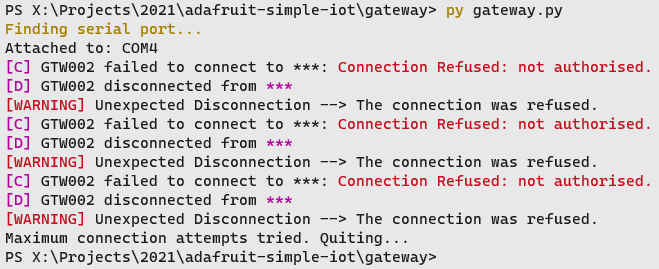
\includegraphics[scale=0.8]{screenshots/connection_failed.png}
    \caption{Connection Failed: Not Authorised}
    \label{fig:gtw-connection-failed}
\end{figure}

Let us run the program again, but this time without the connection of the Arduino as COM port 4. The result is depicted in Figure \ref{fig:gtw-no-com}. Our gateway complains that it found no attached device at the terminal end, so it quits immediately. Later on we will see that, any unexpected disconnection between the gateway and the Arduino will cause our program to terminate without hesitation.

\begin{figure}
    \centering
    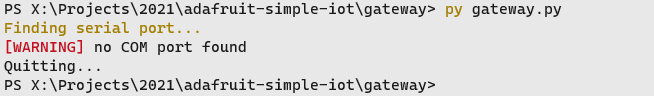
\includegraphics[scale=0.8]{screenshots/no_com.png}
    \caption{No COM port found}
    \label{fig:gtw-no-com}
\end{figure}

\subsubsection{Global Variables and Shared Variables}
\begin{lstlisting}[language=Python, caption= Gateway Program - Variables, escapeinside={(*}{*)}, label=code:gtw-variables]
# ---------- GLOBAL VARIABLES ---------------
block       = False # flag to block thread
exquit      = False # flag to raise disconnect interrupt
greeting    = True  # indicate if this is the first connection
reinit      = False # flag to call init() procedure on reconnect
texceed     = False # indicate if we've reached maximum blocking time
failcount   = 0     # count attempts on fail activity
msg         = ''    # hold buffer message read from serial

# ----------- SHARED-MEMORY -----------------
messageBuffer = queue.Queue()   # holds incoming messages
devicesBuffer = queue.Queue()   # holds outgoing messages
terminate     = False   # control thread termination
scanning      = False   # flag to indicate initial setup
timerexit     = False   # control timer termination
\end{lstlisting}
The next part of our program is reserved for declaring the global and shared variables, as Listing \ref{code:gtw-variables} shows. We have quite a lot variables here, each has it own responsibility on certain aspect of the program, though most of them are involved in the controlling of asynchronous threads. Why thread? The paho-mqtt API offers multiple callbacks that get automatically invoked after a certain action of the MQTT protocol. These threads are, however, asynchronous to the main thread of our program, so we will need these variables to prevent messy debug messages on the console.

Aside from the variables, we have 2 instances of type \texttt{queue} acting as buffers. These queues will ease up the rate of transmitting data and handle multiple incoming messages without hindering other activities in the big while loop. It is important to note that the rate of transmission is NOT unlimited when it comes to Adafruit server:
\begin{quote}
    Adafruit IO's MQTT server imposes a rate limit to prevent excessive load on the service. If a user performs too many publish actions in a short period of time then some of the requests will be rejected and an error message will be published on your /throttle topic. The current rate limit is at most 30 requests per minute for free accounts, 60 per minute with an IO+ account, and expandable via Adafruit IO+ Boost applied to your account.
\end{quote}
You heard the IO, we must have some control in the case the Arduino sends too many data packets in a mimute. The \texttt{deviceBuffer} queue will hold these messages from the Arduino. The Arduino can flood this queue with as many data packets as it wants, because our Gateway program will process these data from the queue one by one independent of the Artduino rate, thus controlling the rate of publishing to the server. On the other hand, the \texttt{messageBuffer} will take on the job of holding messages published by the broker. Its purpose is the same as of the \texttt{deviceBuffer}: prevent the contention occurs inside the big while loop.

\subsubsection{Defining Callbacks}
We will need to define some callbacks that are part of the MQTT API protocol. Some of them serve as debugging, while the others are essential to the gateway functionality. Listing \ref{code:gtw-on-connect} shows the definition of the \texttt{on\_connect()} callback.
\begin{lstlisting}[language=Python, caption= Gateway Program - on\_connect(), escapeinside={(*}{*)}, label=code:gtw-on-connect]
def on_connect(client, userdata, flags, rc):
    if rc != 0: # connection failed
        print(f"{col.cdtag}[C]{col.esc} {GATEWAY_ID} failed to connect to {USERNAME}: {col.bad}{mqtt.connack_string(rc)}{col.esc}")
    else:       # connect successfully
        global greeting
        if greeting:    # the first time this client get connected
            print(f"{col.cdtag}[C]{col.esc} {GATEWAY_ID} connected to {col.user}{USERNAME}{col.esc} with result: {col.good}{mqtt.connack_string(rc)}{col.esc}")
            greeting = False
            global block
            block = False
        else:           # client is making re-connection attempt
            print(f"{col.cdtag}[C]{col.esc} Reconnected to {col.user}{USERNAME}{col.esc} with result: {col.good}{mqtt.connack_string(rc)}{col.esc}")
\end{lstlisting}
The passed in argument \texttt{rc} is used to check the status of connection. If the client failed to connect to the server (\texttt{rc != 0}), then we print out the reason of failure using the method \texttt{connack\_string()} to interpret the reason code. If everything is fine, we continue to see whether the client is making the first connection or a re-connection attempt, and process accordingly.

\begin{lstlisting}[language=Python, caption= Gateway Program - on\_disconnect(), escapeinside={(*}{*)}, label=code:gtw-on-disconnect]
def on_disconnect(client, userdata, rc):
    print(f"{col.cdtag}[D]{col.esc} {GATEWAY_ID} disconnected from {col.user}{USERNAME}{col.esc}")
    if rc != 0:
        print(f"{col.bad}[WARNING]{col.esc} Unexpected Disconnection --> {mqtt.error_string(rc)}")
        global failcount, reinit, scanning
        reinit = True       # the program should do the reinit when get reconnect
        scanning = False    # terminate all activites in the big while loop
        failcount = failcount + 1   # count retrying attempts
\end{lstlisting}
In contrast, Listing \ref{code:gtw-on-disconnect} shows the routine that get called when our client disconnects from the broker. If the disconnection were unexpected (network drops, etc), then we would expect the program to reconnect to the server after a while. The \texttt{reinit} and \texttt{scanning} flag are set to reflect this expectation. We also count the consecutive fail attempts inside this callback for making termination decision on other part of the program.

The next callback shall be the \texttt{on\_message()}, represented in Listing \ref{code:gtw-on-message}. This time we utilize the argument \texttt{userdata} which is automatically passed in by the MQTT implementation. The \texttt{userdata} is an object reserved for whatever purpose the developers want to pass custom data into callbacks that accept the argument. Here, we will use it to filter out the owning messages (messages that are sent and received by the same client). Before publishing any message to the server, we set the \texttt{userdata} object to hold an array of string where the first string is the payload and the second string is the topic name. This instance of the \texttt{userdata} object will then get passed into any callback that has a parameter accepting the object, including our \texttt{on\_message()} callback. It is then the job of the \texttt{on\_message()} function to use the passed in argument to check if the received message is the same as one hold by the \texttt{userdata}.
\begin{lstlisting}[language=Python, caption= Gateway Program - on\_message(), escapeinside={(*}{*)}, label=code:gtw-on-message]
def on_message(client, userdata, message):
    msgv = message.payload.decode()                         # get message value
    msgt = message.topic[message.topic.find('.') + 1:]      # get message topic
    # filter out owning message
    if msgv == userdata[0] and msgt == userdata[1]:
        global block    # release block
        block = False
    else:
        print(f"{col.mestag}[M]{col.esc} Received {col.message}{msgv}{col.esc} on topic: {col.topic}{msgt}{col.esc}")
        # if receive offline instruct from the broker
        if (msgt == STAT_TOPIC and msgv == "offline"):
            global exquit
            exquit = True
        
        # otherwise add message to the buffer
        else:
            if scanning: messageBuffer.join()
            messageBuffer.put((msgt, msgv))
\end{lstlisting}
The listing reveals more than just the filtering-message thing. Here we also handle the case where we receive an \textbf{offline} message from the topic \textbf{gtw-status}. The flag \texttt{exquit} is set to indicate we should clean up and terminate our program.

The 2 last callbacks involving in this program are shown in Listing \ref{code:gtw-on-pubsub}. For the publishing, we just simply check the topic we are sending message to and change the debug message accordingly. The subscribing, on the other hand, has a job to release the thread lock hold by the variable \texttt{block}. Why blocking thread? This has to do with the order that the debug messages appear on the console. Normally, the subscribing protocol is very fast and less error-prone, so the subscription message will usually get printed first, even before the successful connection message get printed. Blocking is put in here to make the debug console more intuitive.
\begin{lstlisting}[language=Python, caption= Gateway Program - on\_publish() and on\_subscribe(), escapeinside={(*}{*)}, label=code:gtw-on-pubsub]
def on_publish(client, userdata, mid):
    if "get" in userdata[1]:
        print(f"Fetching {col.stage}latest data{col.esc} from {userdata[1][:-4]}...")
    elif userdata[1] is STAT_TOPIC:
        print(f"{GATEWAY_ID} has set its status to {col.stage}{userdata[0]}{col.esc}")
    else:
        print(f"{col.pubtag}[P]{col.esc} Published {col.pubtag}{userdata[0]}{col.esc} to: {col.topic}{userdata[1]}{col.esc}")

def on_subscribe(client, userdata, mid, granted_qos):
    global block
    print(f"{col.subtag}[S]{col.esc} Subscribed to: {col.topic}{userdata}{col.esc}")
    block = False   # release block
\end{lstlisting}

Before moving on, let see how a successful connection to the server looks like. Figure \ref{fig:gtw-normal} illustrates a normal gateway connection. We start off finding the COM port where the Arduino attachs to, and then try to establish a connection to the server. On successful connection, we start fetching latest data from the topics in the subscribe list. Finally, we publish an \textbf{online} message to the \textbf{gtw-status} topic before jump into the forever while loop.

\begin{figure}
    \centering
    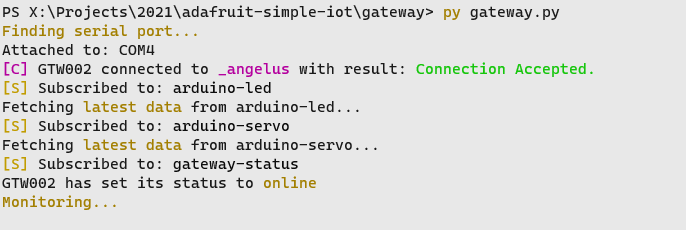
\includegraphics[scale=0.8]{screenshots/normal.png}
    \caption{A successful gateway connection.}
    \label{fig:gtw-normal}
\end{figure}

\subsubsection{Utility Functions}
Let's talk a little bit about some helpful functions used throughout the program. There are quite a lot of them, but the document only lists those that worth mentioning. Listing \ref{code:gtw-init} shows the \texttt{init()} routine, which is responsible for subscribing to the required topics and getting latest data upon each successful subscription. This function will also come in handy when our client get unexpected disconnection and then wish to resubscribe to the topics after reconnecting to the server. The function also illustrates the use of \texttt{userdata} object, the */get solution for latest data fetching, and the variable \texttt{block} to synchronize debug message. The function finishes off setting the gateway status to \textbf{online} by publishing the according message to the \texttt{STAT\_TOPIC}.
\begin{lstlisting}[language=Python, caption= Gateway Program - init() function, escapeinside={(*}{*)}, label=code:gtw-init]
def init():
    global gtw, ser
    # subscribe to required topics
    # -----
    for top in SUBSCRIBE_TOPICS:
        global block
        block = True    # raise a block flag
        gtw.user_data_set(top)
        gtw.subscribe(topic=f"{USERNAME}/feeds/{GROUP_KEY}.{top}", qos=SUB_QOS)
        while block:
            pass        # block thread until fully subscribed
        # fetch latest data, except for the 'status' topic
        if top is not STAT_TOPIC:
            publish('', f"{top}/get")

    # publish 'online' to status feed
    # ------
    publish("online", STAT_TOPIC)
\end{lstlisting}

Listing \ref{code:gtw-publish} shows the implementation of the wrapper \texttt{publish()} function. We need a wrapper here because there are a couple things that need be done besides publishing. The method \texttt{wait\_for\_publish()} that comes right after the execution of the \texttt{publish()} method has the effect of synchronization. It will block the current thread until the callback \texttt{on\_publish()} get invoked. We also have to manually blocking the current thread if we sending message to the topic we subscribe to. The client must detect the owing message and filter it out before it can continue its execution. This blocking might take forever, although it may only happen in rare case. Even so, the function is provided with mechanism to automatically release the block if the waiting time exceeds the value of the constant \texttt{TIME\_OUT}. We achieve this by launching a separate thread that acts like a countdown timer. The shared variable \texttt{texceed} is the flag that will be set to indicate if the waiting time is too long. The timer routine that run on the separate is shown in Listing \ref{code:gtw-timer}.
\begin{lstlisting}[language=Python, caption= Gateway Program - publish() function, escapeinside={(*}{*)}, label=code:gtw-publish]
def publish(payload, topic):
    global gtw
    gtw.user_data_set([payload, topic])
    pub = gtw.publish(f"{USERNAME}/feeds/{GROUP_KEY}.{topic}", payload, PUB_QOS)
    pub.wait_for_publish()
    # if publishing to subscribed topic
    if topic in SUBSCRIBE_TOPICS:
        global block, texceed, timerexit
        # then block thread until having fully filtered out the owning message
        block = True
        texceed = False
        timerexit = False
        taskTiming = threading.Thread(target=timer) # only block for the maximum time decided by the timer
        taskTiming.start()
        while block:
            if texceed: # timer exceeds
                print(f"{col.bad}[WARNING]{col.esc} Reached maximum waiting time for validating own message. Continuing...")
                taskTiming.join()
                block = False
        if taskTiming.is_alive():   # join the separate timer thread
            timerexit = True
            taskTiming.join()
\end{lstlisting}
One of the most buggy thing about multi-threaded programming is that we usually forget to join the separate thread. Our \texttt{publish()} function does its best to join any thread its launch on every possible exit path.
\begin{lstlisting}[language=Python, caption= Gateway Program - timer() function, escapeinside={(*}{*)}, label=code:gtw-timer]
def timer():
    global texceed
    count = 0
    while True:
        if timerexit:
            break
        time.sleep(1.0)
        count = count + 1
        if count == TIME_OUT:
            texceed = True
            break
\end{lstlisting}

The implementation of \texttt{timer()} is pretty straightforward. We use the built-in \texttt{sleep()} method to count the elapsed second. There are 2 possible ways our timer can terminate: whther the gateway filters out its owning message on time or it does not. Either way, we make sure the while loop is broken so that the thread can exit properly. The shared data \texttt{timerexit} is used here to signal the if the gateway has filtered out the owing message on time.

\begin{lstlisting}[language=Python, caption= Gateway Program - watcher() function, escapeinside={(*}{*)}, label=code:gtw-watcher]
def watcher():
    global exquit, ser
    while True:
        if terminate:
            ser.close()
            break
        try:
            driver()
        except SerialException:
            print(f"{col.bad}[WARNING]{col.esc} Lost connection to serial. Quitting...")
            ser.close()
            exquit = True
            break
\end{lstlisting}

Finally, there is another co-routine that monitors the incoming data from the Arduino, the \texttt{watcher()} function (Listing \ref{code:gtw-watcher}). Much like the timer, we have a shared variable \texttt{terminate} to signal if the our thread should exit on command. As long as this variable is not asserted, the watcher will call the \texttt{driver()} function repeatedly to check for character sequences at the terminal. There is another exit point for the watcher: the Arduino get disconnected unexpectedly. When this happens, the \texttt{driver()} will raise an exception, and the watcher signals our main thread to terminate the gateway program.

\subsubsection{Main Script}
It's time to put everything we've come through together. Listing \ref{code:gtw-main} shows the main script of our gateway program.
\begin{lstlisting}[language=Python, caption= Gateway Program, escapeinside={(*}{*)}, label=code:gtw-main]
# ------------------ MAIN GATEWAY SCRIPT -------------------

# instantiate a gateway client and setup some options
# -----
gtw = mqtt.Client(client_id=GATEWAY_ID)
gtw.tls_set_context()
gtw.username_pw_set(username=USERNAME, password=PASSWORD)
gtw.will_set(f"{USERNAME}/feeds/{GROUP_KEY}.{STAT_TOPIC}", 'offline') (*\label{code:gtw-main:will}*)

# register callbacks
# -----
gtw.on_connect = on_connect
gtw.on_disconnect = on_disconnect
gtw.on_publish = on_publish
gtw.on_subscribe = on_subscribe
gtw.on_message = on_message

# connect to serial com port
# -----
try:
    print(f"{col.stage}Finding serial port...{col.esc}")
    ser = serial.Serial(getport(), BAUDRATE)
except SerialException:
    print("Quitting...")
    exit(1)

# start external thread
# -----
taskWatching = threading.Thread(target=watcher)
taskWatching.start()

# connect to the broker
# -----
gtw.connect(host=HOST_NAME, port=HOST_PORT)

# start recording change
# -----
gtw.loop_start()

# block thread until having connected successfully
# -----
block = True
failcount = 0
while block:
    if failcount == MAX_FAILED_ATTEMPTS:
        terminate = True
        taskWatching.join()
        gtw.disconnect()
        time.sleep(0.1)
        print("Maximum connection attempts tried. Quiting...")
        exit(1)

# subscribe to required topics & publish 'online' to status feed
# -----
init()

# monitor external devices
# -----
print(f"{col.stage}Monitoring...{col.esc}")
scanning = True
try:
    while True: (*\label{code:gtw-main:big-while}*)
        # do the init procuder again on reconnect
        if gtw.is_connected and reinit:
            init()
            reinit = False
            scanning = True
        
        # if there still be data waiting to be published in the buffer
        while gtw.is_connected and not reinit and not devicesBuffer.empty():
            tup = devicesBuffer.get()
            publish(tup[1], tup[0])
            devicesBuffer.task_done()

        # if there still be message waiting to be processed in the buffer
        while not messageBuffer.empty():
            tup = messageBuffer.get()
            ser.write(f"!{SUBSCRIBE_TOPICS.index(tup[0])}:{tup[1]}#".encode())
            messageBuffer.task_done()

        # constantly check if there is a terminate signal from broker
        if exquit:
            raise KeyboardInterrupt


        # scan delay
        time.sleep(SCAN_DELAY)

# disconnect on cancel
# -----
except KeyboardInterrupt:   (*\label{code:gtw-main:keyboard-except}*)
    # terminate watcher thread
    print("Terminating watcher...")
    terminate = True
    taskWatching.join(timeout=1.0)
    publish("offline", STAT_TOPIC)
    res = gtw.disconnect()
    time.sleep(0.1) # delay a small amount of time for on_disconnect() callback
    print(f"Disconnect Status: {col.good if res == 0 else col.bad}{mqtt.error_string(res)}{col.esc}")
\end{lstlisting}
I believe with the comment in between, the listing is self-conveying. There is one point that need mentioned, however. Because our gateway will run forever on end inside the big while loop (starting at line \ref{code:gtw-main:big-while}), if we want to safely terminate the program (via Ctrl + C, for example), we should wrap the big loop in side a \texttt{try} block and have an exception handler to terminate our program clean and neat (line \ref{code:gtw-main:keyboard-except}).

\subsection{Gateway Conclusion}
So that's how we implement the gateway. I especially focus on making the program more reliable, with various unexpected behaviour handled properly. Our program, unfortunately, has a small bug. This bug is not attributed to the developer (of course), but rather it is because we lack an useful feature of the MQTT on Adafruit: the \textit{will set}. If a client registers a backup message (a will) on a topic, then when this client unexpectedly disconnects from the server, the broker will automatically publish this registered message to that topic. An example use of will set can be found at line \ref{code:gtw-main:will} of the main program above. Here we tell the broker that if the gateway unexpectedly looses connection to the server, then the broker should publish the message \textbf{offline} to the \textbf{gtw-status} topic, to indicate that the gateway has (badly) gone offline. But we are unlucky because the Adafruit server does not provide such a handy feature, and we should start to smell trouble. If our gateway unexpectedly gets disconnected from the server, then we have no way to publish the offline status without the help of will set. This means at some point in the lifetime of our gateway, the status topic shows that our gateway is online, but in fact it may not be working due to unexpected connection error. Our gateway might find its own way to reconnect to the server after a fatal disconnection, but still this is unacceptable for system that demands higher level of reliability. If this is the case, then we should consider state-of-the-are brokers like the Eclipse Mosquitto or the HiveMQ. These come with the MQTT v5.0 support, which is much more suitable for critical IoT projects. The Adafruit, however, has its own advantages. It provides beautiful interface monitors called \textit{dashboards} to help us organize the components involved in the system (section \ref{section:server}). Also, the security on the Adafruit is extremely reliable. If the user's private key get accidentally leaked (public source code on Github, for example), then the user automatically receives an email from the Adafruit team with a friendly warning. All and all, Adafruit should be a place of choice for education and small-scaled projects.
\clearpage